\documentclass[11pt,letterpaper]{report}
\usepackage[pdftex]{graphicx}
\usepackage[version=3]{mhchem}

\newcommand{\HRule}{\rule{\linewidth}{0.5mm}}
\setlength{\topmargin}{-.7in}
\setlength{\leftmargin}{-.7in}
\setlength{\textheight}{9in}
\setlength{\oddsidemargin}{0in}
\setlength{\textwidth}{6.25in}


\begin{document}

\begin{titlepage}
\begin{center}

\textsc{\Large Grossmont College - Chemistry 141}\\[1.5cm]
\textsc{\Large Lab 3}\\[0.5cm]

\HRule \\[0.4cm]
{ \LARGE \bfseries Copper Reactions}\\[0.5cm]

\HRule \\[1.5cm]

\begin{minipage}{0.4\textwidth}
\begin{flushleft} \large
\emph{Author:}\\
Cameron \textsc{Carroll}
\end{flushleft}
\end{minipage}
\begin{minipage}{0.4\textwidth}
\begin{flushright} \large
\emph{Instructor \& Class:}\\
Judy \textsc{George} - 141 (8844)
\end{flushright}
\end{minipage}\\[2cm]

{\large \today}

\vfill

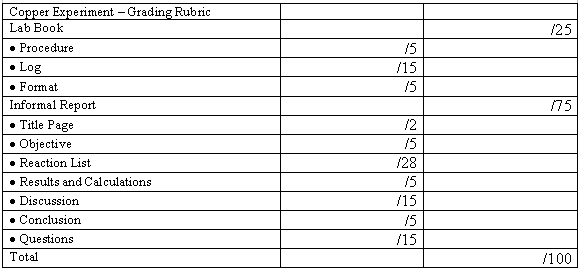
\includegraphics{./copper_rxn_rubric.png}\\[1cm]



\end{center}
\end{titlepage}
\pagebreak

\section*{Objective}
The purpose of this experiment is to explore the law of conservation of mass and energy. This natural law, discovered by Lvoisier, theoretically allows a sample of copper to be transformed into a number of different compounds, and back into copper without creating or destroying any mass in the process. The exploration is a seven step process, transmuting copper into a different substance in each.

\section*{Reaction List}
\begin{enumerate}
\item \ce{Cu_{(s)} + 4HNO3_{(aq)} -> Cu(NO3)2_{(aq)} + 2NO2_{(g)} + 2H2O_{(l)}}
\begin{itemize}
\item \textsc{Reaction Type:} Reduction - Oxidation
\item \textsc{Expected Yield:} 0.664 grams
\item \textsc{Stoichiometry:} $0.00323 \text{ mol \ce{Cu} } ( \frac{\text{1 mol \ce{Cu(NO3)2}}}{\text{1 mol \ce{Cu}}} ) ( \frac{\text{205.55 \text{ grams} \ce{Cu(NO3)2}}}{\text{1 mol \ce{Cu(NO3)2}}} ) = 0.664 \text{ grams}$
\end{itemize}
\item \ce{Cu^2+_{(aq)} + 2(OH)^{-}_{(aq)} -> Cu(OH)2_{(s)}}
\begin{itemize}
\item \textsc{Reaction Type:} Precipitation
\item \textsc{Expected Yield:} 0.315 grams
\item \textsc{Stoichiometry:} $0.00323 \text{ mol \ce{Cu(NO3)2} } ( \frac{\text{1 mol \ce{Cu(OH)2}}}{\text{1 mol \ce{Cu(NO3)2}}} ) ( \frac{\text{97.57 \text{ grams} \ce{Cu(OH)2}}}{\text{1 mol \ce{Cu(OH)2}}} ) = 0.315 \text{ grams}$
\end{itemize}
\item \ce{Cu(OH)2_{(s)} -> CuO_{(s)} + H2O_{(l)}}
\begin{itemize}
\item \textsc{Reaction Type:} Decomposition
\item \textsc{Expected Yield:} 0.257 grams
\item \textsc{Stoichiometry:} $0.00323 \text{ mol \ce{Cu(OH)2} } ( \frac{\text{1 mol \ce{CuO}}}{\text{1 mol \ce{Cu(OH)2}}} ) ( \frac{\text{79.55 \text{ grams} \ce{CuO}}}{\text{1 mol \ce{CuO}}} ) = 0.257 \text{ grams}$
\end{itemize}
\item \ce{CuO_{(s)} + H2SO4_{(aq)} -> CuSO4_{(aq)} + H2O_{(l)}}
\begin{itemize}
\item \textsc{Reaction Type:} Acid/Base Neutralization
\item \textsc{Expected Yield:} 0.516 grams
\item \textsc{Stoichiometry:} $0.00323 \text{ mol \ce{CuO} } ( \frac{\text{1 mol \ce{CuSO4}}}{\text{1 mol \ce{CuO}}} ) ( \frac{\text{159.6 \text{ grams} \ce{CuSO4}}}{\text{1 mol \ce{CuSO4}}} ) = 0.516 \text{ grams}$
\end{itemize}
\item \ce{Cu^2+_{(aq)} + (PO4)^{3-}_{(aq)} -> Cu3(PO4)2_{(s)}}
\begin{itemize}
\item \textsc{Reaction Type:} Double Displacement
\item \textsc{Expected Yield:} 0.41 grams
\item \textsc{Stoichiometry:} $0.00323 \text{ mol \ce{CuSO4} } ( \frac{\text{1 mol \ce{Cu3(PO4)2}}}{\text{1 mol \ce{CuSO4}}} ) ( \frac{\text{380.6 \text{ grams} \ce{Cu3(PO4)2}}}{\text{1 mol \ce{Cu3(PO4)2}}} ) = 0.410 \text{ grams}$
\end{itemize}
\item \ce{Cu3(PO4)2_{(s)} -> Cu_{(aq)} + (PO4)^{3-}_{(aq)}}
\begin{itemize}
\item \textsc{Reaction Type:} Double Displacement
\item \textsc{Expected Yield:} 0.432 grams
\item \textsc{Stoichiometry:}  $0.00107 \text{ mol \ce{Cu3(PO4)2} } ( \frac{\text{1 mol \ce{CuCl2}}}{\text{1 mol \ce{Cu3(PO4)2}}} ) ( \frac{\text{134.5 \text{ grams} \ce{CuCl2}}}{\text{1 mol \ce{CuCl2}}} ) = 0.432 \text{ grams}$
\end{itemize}
\item \ce{2Al_{(s)} + Cu^2+_{(aq)} -> Cu_{(s)} + 2Al+_{(aq)}}\\
\begin{itemize}
\item \textsc{Reaction Type: Reduction - Oxidation} 
\item \textsc{Expected Yield:} 0.205 grams
\item \textsc{Stoichiometry:} $0.00323 \text{ mol \ce{CuCl2} } ( \frac{\text{1 mol \ce{Cu}}}{\text{1 mol \ce{CuCl2}}} ) ( \frac{\text{63.55 \text{ grams} \ce{Cu}}}{\text{1 mol \ce{Cu}}} ) = 0.205 \text{ grams}$
\end{itemize}
\end{enumerate}

\section*{Results \& Calculations}
\begin{itemize}
\item \textsc{Expected Yield:} 0.205 grams
\item \textsc{Actual Yield:} 0.699 grams
\item \textsc{Percent Yield:} 341\%
\end{itemize}

\section*{Discussion}
The resultant compound had a clay-like consistency, and dried to a dull powder. This difference in appearance may be because the metal was in a polished form before, and a raw material form after the reaction series. The sample had silver specks at the top, which confirms that there was still some aluminum. This is a result of being rushed during the process of dissolving aluminum with hydrochloric acid; Not enough acid was used to finish the reaction, causing the sample size to be larger. In addition to this error, the nature of the experiment means that much debris and waste-solution is generated, causing a lot of contamination throughout each process; The recapturing of copper can theoretically be perfect, but in reality there are inefficiencies. 

\section*{Conclusion}
The mass of the reclaimed sample was 0.699 grams, 341\% higher than the theoretical yield of 0.205 grams. This is due to inherent inefficiencies in the laboratory processes, as well as some human error. The exploration of the law of conservation of mass \& energy succeeds because it is clear that all of the copper has gone either into the waste solutions or has been reclaimed.

\section*{Post-Lab Questions}
\begin{enumerate}
\item $3.50 \text{kg \ce{Cu}} (\frac{68.3 \text{g}}{100 \text{g}}) (\frac{100 \text{g}}{90 \text{g}})  = 5.69 \text{kg \ce{Cu}}$
\item Prepare copper (II) nitrate from copper(II) chloride
\begin{itemize}
\item Add \ce{NaNO3}.
\item \ce{CuCl2_{(aq)} + NaNO3_{(aq)} -> Cu(NO3)2_{(aq)} + NaCl_{(aq)}}
\item Copper (II) sample can be isolated by following the series of reactions starting at reaction 2.
\end{itemize}
\item Prepare copper (II) hydroxide from copper (II) sulfate
\begin{itemize}
\item Add \ce{H2O}
\item \ce{CuSO4_{(aq)} + 2H2O_{(l)} -> Cu(OH)2_{(s)} + H2SO4_{(aq)}}
\item Follow lab procedures starting from reaction 3.
\end{itemize}
\end{enumerate}


\end{document}